\documentclass[a4paper,presentation]{beamer}


\usepackage[utf8]{inputenc}
\usepackage{verbatim}
\usepackage{graphicx}
\usepackage{color}
\usepackage{hyperref}
\usepackage{url}
\usepackage{tikz}
\usepackage{moreverb}
\usepackage{fancyvrb}
\usepackage{minted}


\tikzset{
  every overlay node/.style={
    draw=white,fill=white,anchor=north west,
  },
  every overlay node border/.style={
    draw=black,fill=white,anchor=north west,rounded corners,
  },
}
% Usage:
% \tikzoverlay at (-1cm,-5cm) {content};
% or
% \tikzoverlay[text width=5cm] at (-1cm,-5cm) {content};
\def\tikzoverlay{%
   \tikz[baseline,overlay]\node[every overlay node]
}%
\def\tikzoverlayborder{%
   \tikz[baseline,overlay]\node[every overlay node border]
}%

\def\Put(#1,#2)#3{\leavevmode\makebox(0,0){\put(#1,#2){#3}}}

\hypersetup{colorlinks=true, linkcolor=black, urlcolor=blue}
\usetheme{boxes}
\setbeamertemplate{itemize items}[circle]
\beamertemplatenavigationsymbolsempty
\setbeamertemplate{sections/subsections in toc}[circle]

\usepackage{pifont}
\newcommand{\cmark}{\ding{51}}%
\newcommand{\xmark}{\ding{55}}%

\title{Gradient Boosted Regression Trees}

\date{}

\begin{document}


% Title slide =================================================================

\begin{frame}

\titlepage

\vspace{-3cm}

\begin{figure}
  \centering
    
\includegraphics[scale=.6]{./images/scikit-learn-logo.pdf}
\end{figure}

\vspace{0.2cm}
  \begin{center}
    {\small Material:
    \href{https://github.com/pprett/pydata-gbrtm-tutorial}{https://github.com/pprett/pydata-gbrt-tutorial}}\\
  \end{center}
\vspace{0.2cm}

\begin{columns}[T]
\begin{column}{.48\textwidth}

\centering
Peter Prettenhofer (\href{https://twitter.com/pprett}{@pprett})\\
{\small\it DataRobot}

\end{column}
\begin{column}{.48\textwidth}

\centering
Gilles Louppe (\href{https://twitter.com/glouppe}{@glouppe})\\
{\small\it Université de Liège, Belgium}

\end{column}
\end{columns}


\end{frame}


% Motivation =====================================================================

\begin{frame}{Motivation}
\begin{figure}
  \centering
    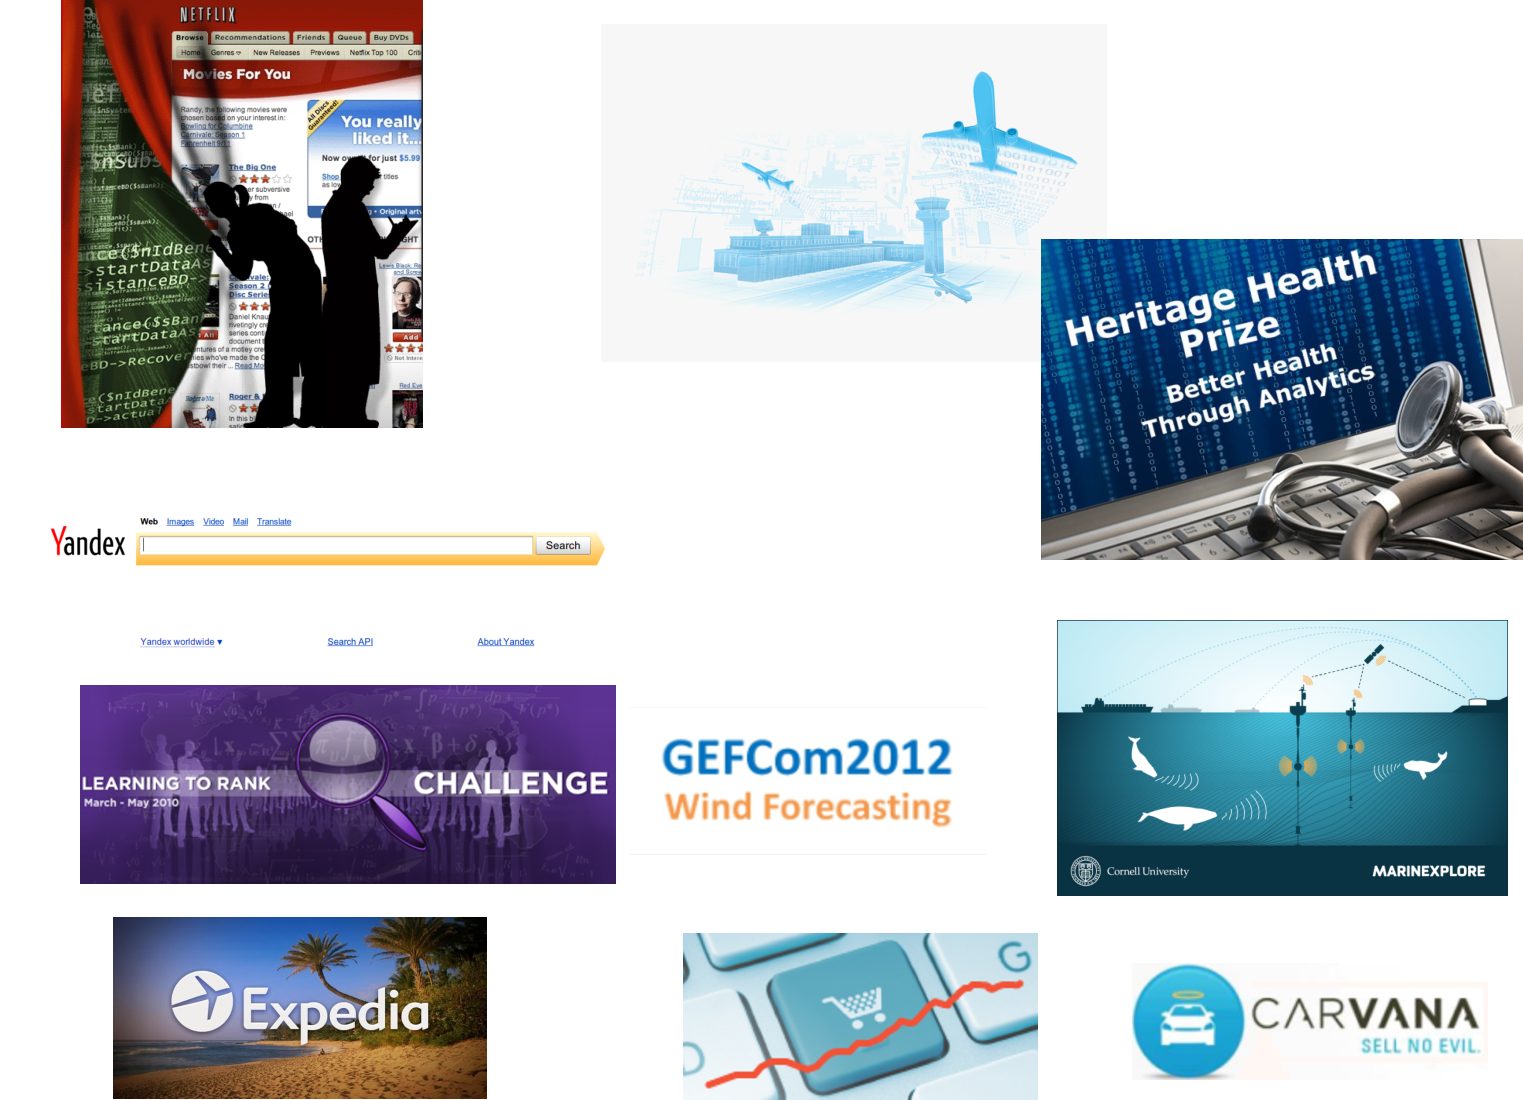
\includegraphics[scale=0.4]{./images/motivation/motivation.pdf} \pause
    \Put(-200,200){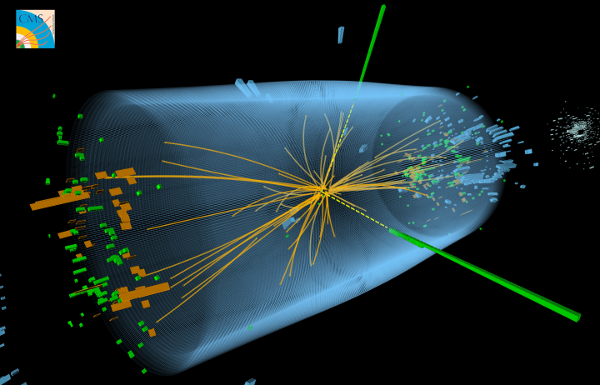
\includegraphics[scale=0.225]{./images/motivation/gammagamma-small.png}}
\end{figure}
\end{frame}

% Outline =====================================================================
\begin{frame}
  \frametitle{Outline}
  \tableofcontents
\end{frame}

% About Us =====================================================================

\begin{frame}{About us}
\begin{columns}[t]

\begin{column}[T]{0.5\textwidth}
\begin{block}{Peter}
    \begin{itemize}
      \item \href{https://twitter.com/pprett}{@pprett}
      \item Python \& ML $\sim$ 6 years
      \item sklearn dev since 2010
    \end{itemize}
\end{block}
\begin{block}{Gilles}
    \begin{itemize}
      \item \href{https://twitter.com/glouppe}{@glouppe}
      \item PhD student (Liège, Belgium)
      \item sklearn dev since 2011\\
        \textit{Chief tree hugger}
    \end{itemize}
\end{block}
\end{column}

\begin{column}[T]{0.45\textwidth}

\begin{figure}
  \centering
    \vspace{-1cm}
    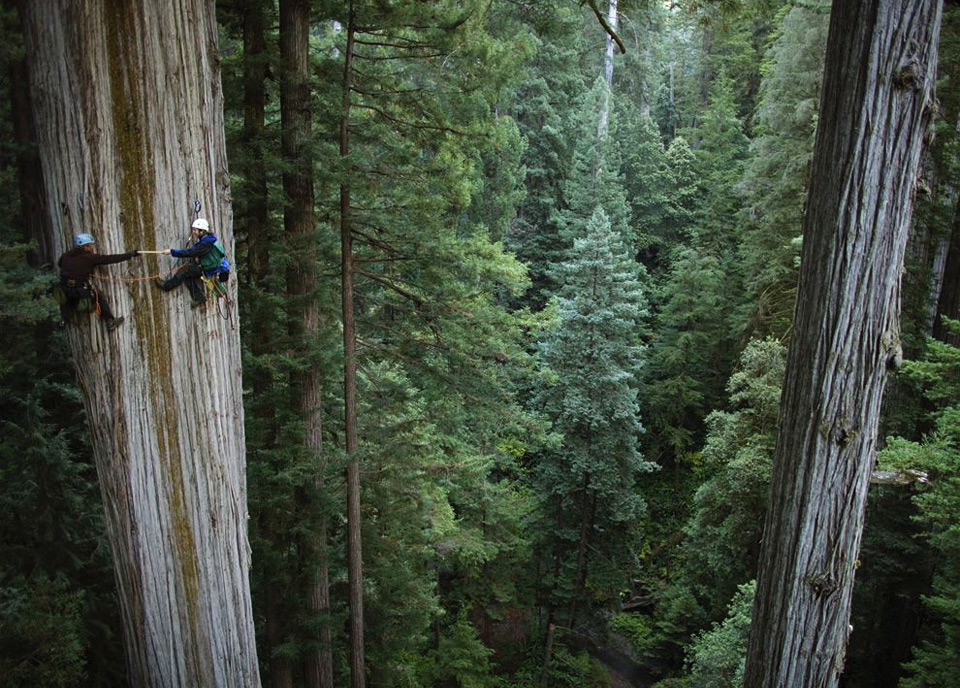
\includegraphics[scale=0.3]{./images/tree-climbers.jpg}
\end{figure}
\end{column}
\end{columns}
\end{frame}


% Outline =====================================================================

\AtBeginSection[]
{
\begin{frame}
  \frametitle{Outline}
  \tableofcontents[currentsection]
  % Die Option [pausesections]
\end{frame}
}

% ML 101 =====================================================================
\section{Basics}

\begin{frame}{Machine Learning 101}
  \begin{itemize}
  \item Data comes as...
    \begin{itemize}
        \vspace{0.2cm}
        \item A set of examples $\{(\mathbf{x}_i, y_i) | 0 \leq i < \text{n\_samples}\}$, with
        \vspace{0.2cm}
        \item Feature vector $\mathbf{x} \in \mathbb{R}^\text{n\_features}$, and
        \vspace{0.2cm}
        \item Response $y \in \mathbb{R}$ (regression) or $y \in \{-1, 1\}$ (classification)
    \end{itemize}
  \vspace{0.5cm}
  \item Goal is to...
    \begin{itemize}
        \vspace{0.2cm}
        \item Find a function $\hat{y} = f(\mathbf{x})$
        \vspace{0.2cm}
        \item Such that error $L(y, \hat{y})$ on new (unseen) $\mathbf{x}$ is minimal
        \vspace{0.5cm}
    \end{itemize}
  \end{itemize}
  \vspace{-0.5cm}
  \begin{figure}
      
\includegraphics[scale=0.2]{./images/ml-course.png}
    \end{figure}
\end{frame}

\begin{frame}{Classification and Regression Trees [Breiman et al, 1984]}

\begin{figure}
   \centering
      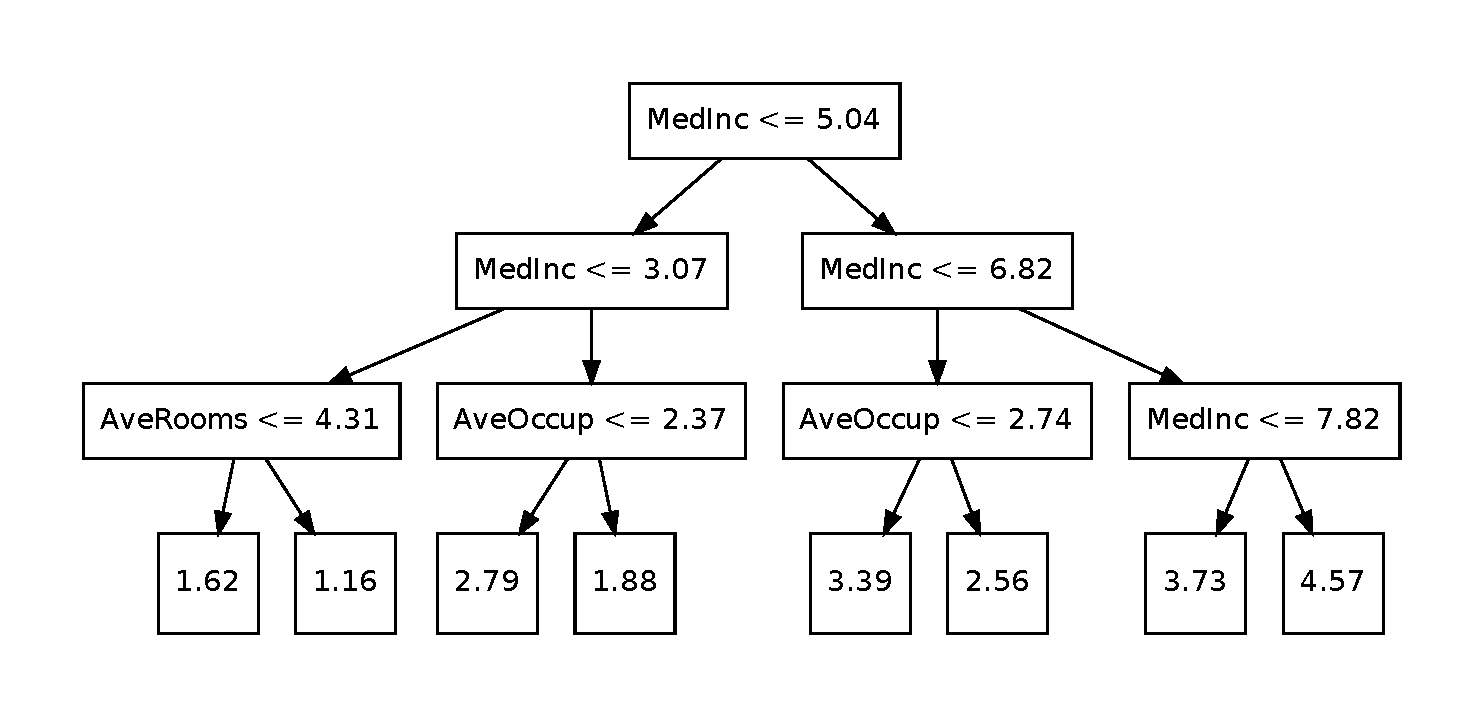
\includegraphics[width=1.0\textwidth]{./images/decision_tree.pdf}
\end{figure}

% sklearn footer
\tikzoverlay[text width=10cm] at (-0.2cm, 0.1cm) {
\begin{columns}[c]
\begin{column}{0.2\textwidth}
    \begin{figure}
      
\includegraphics[width=2em]{./images/scikit-learn-logo-thumb.png}
    \end{figure}
\end{column}
\begin{column}{1.0\textwidth}
    \vspace{-0.5cm}\hspace{-0.5cm}{\footnotesize \texttt{sklearn.tree.DecisionTreeClassifier|Regressor}}
\end{column}
\end{columns}
};

\end{frame}

\begin{frame}{Function approximation with Regression Trees}

\begin{figure}
  \centering
    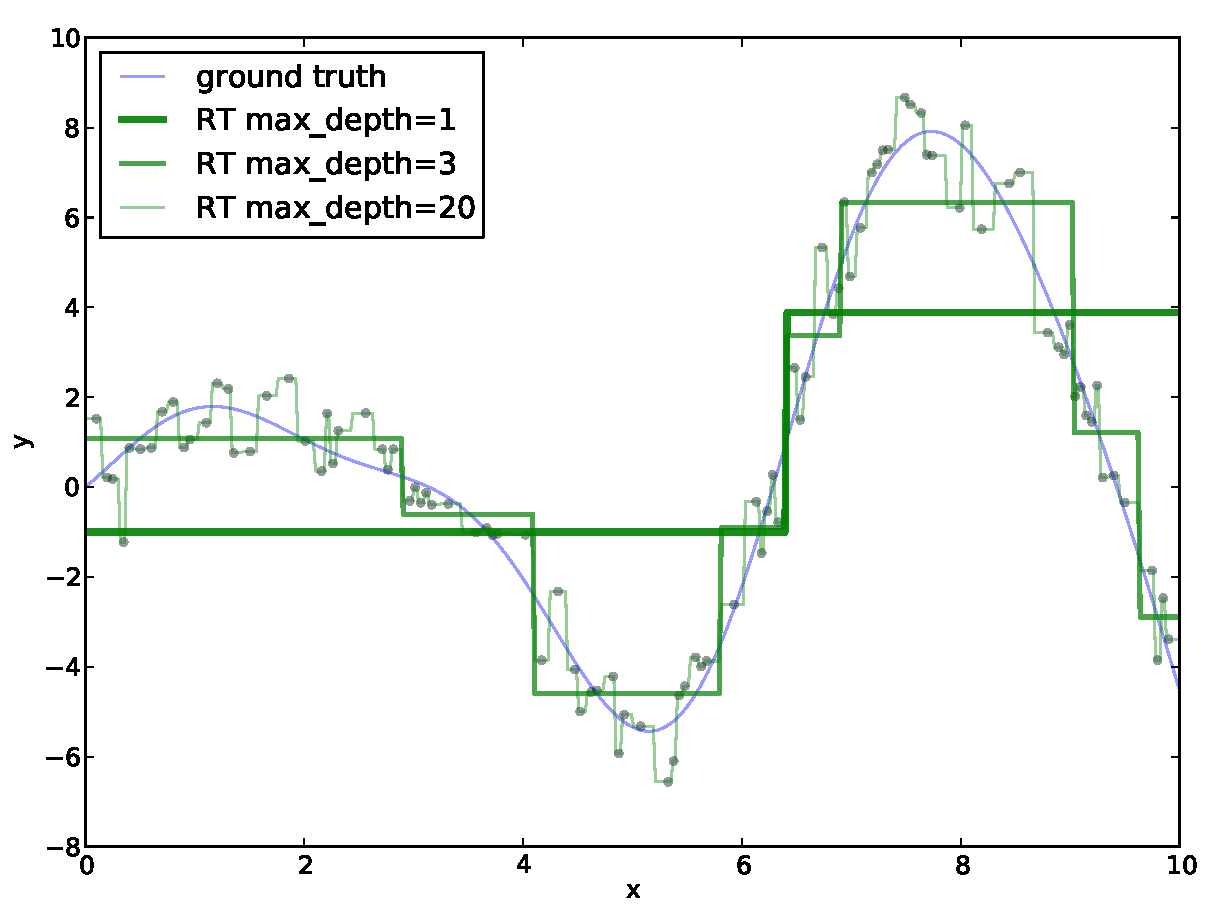
\includegraphics[width=1.0\textwidth]{./images/func_approx_tree_3.pdf}
\end{figure}


\onslide<2->{
\tikzoverlayborder[text width=9cm] at (1cm,6cm) {
\begin{alertblock}{Deprecated}
\begin{itemize}
   \item Nowadays seldom used alone
   \item Ensembles: Random Forest, Bagging, or Boosting (see \texttt{sklearn.ensemble})
\end{itemize}
\end{alertblock}
};
}
\end{frame}


\section{Gradient Boosting}
% What is GBRT? =====================================================================

\begin{frame}{Gradient Boosted Regression Trees}
%Flexible non-parametric classification and regression technique
\begin{block}{Advantages}
  {\footnotesize
      \begin{itemize}
        \item Heterogeneous data (features measured on different scale)
        \item Supports different loss functions (e.g. huber)
        \item Automatically detects (non-linear) feature interactions
        %\item State-of-the-art predictive accuracy, but still
        %\item Interpretable
      \end{itemize}
  }
\end{block}
\begin{block}{Disadvantages}
  {\footnotesize
      \begin{itemize}
        \item Requires careful tuning
        \item Slow to train (but fast to predict)
        \item Cannot extrapolate
      \end{itemize}
  }
\end{block}

\tikzoverlay[text width=5cm] at (7.28cm, 3.67cm) {
\begin{figure}
  \centering
    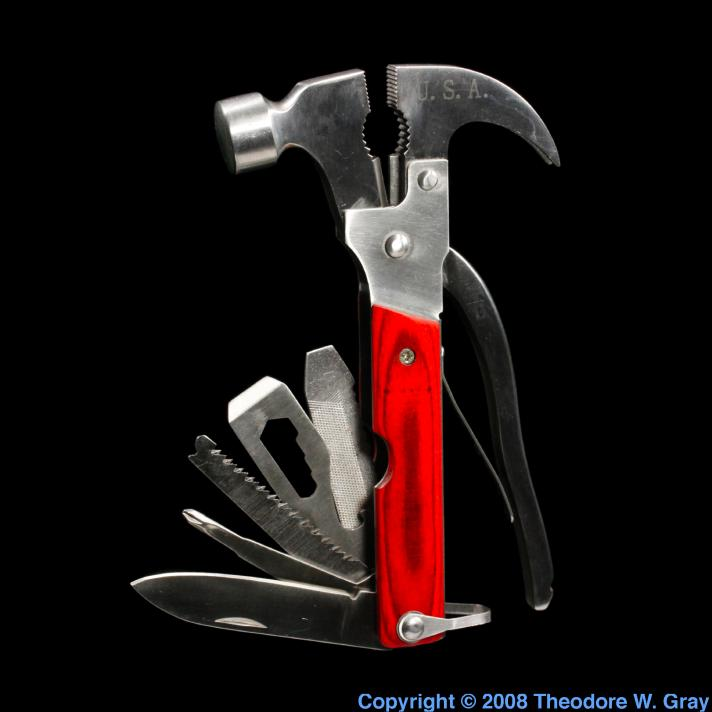
\includegraphics[scale=0.15]{./images/swiss-army-hammer.jpg}
\end{figure}
};
\end{frame}

% Boosting =====================================================================
\begin{frame}{Boosting}
  %\vspace{0.75cm}
  %Can we build a strong learner from multiple weak learners?
    % Posed by Kearns and Valiant in 1988
    \begin{block}{AdaBoost [Y. Freund \& R. Schapire, 1995]}
        \begin{itemize}
           \item Ensemble: each member is an expert on the errors of its predecessor
           \item Iteratively re-weights training examples based on errors
        \end{itemize}
        \vspace{-0.2cm}
        \begin{figure}
          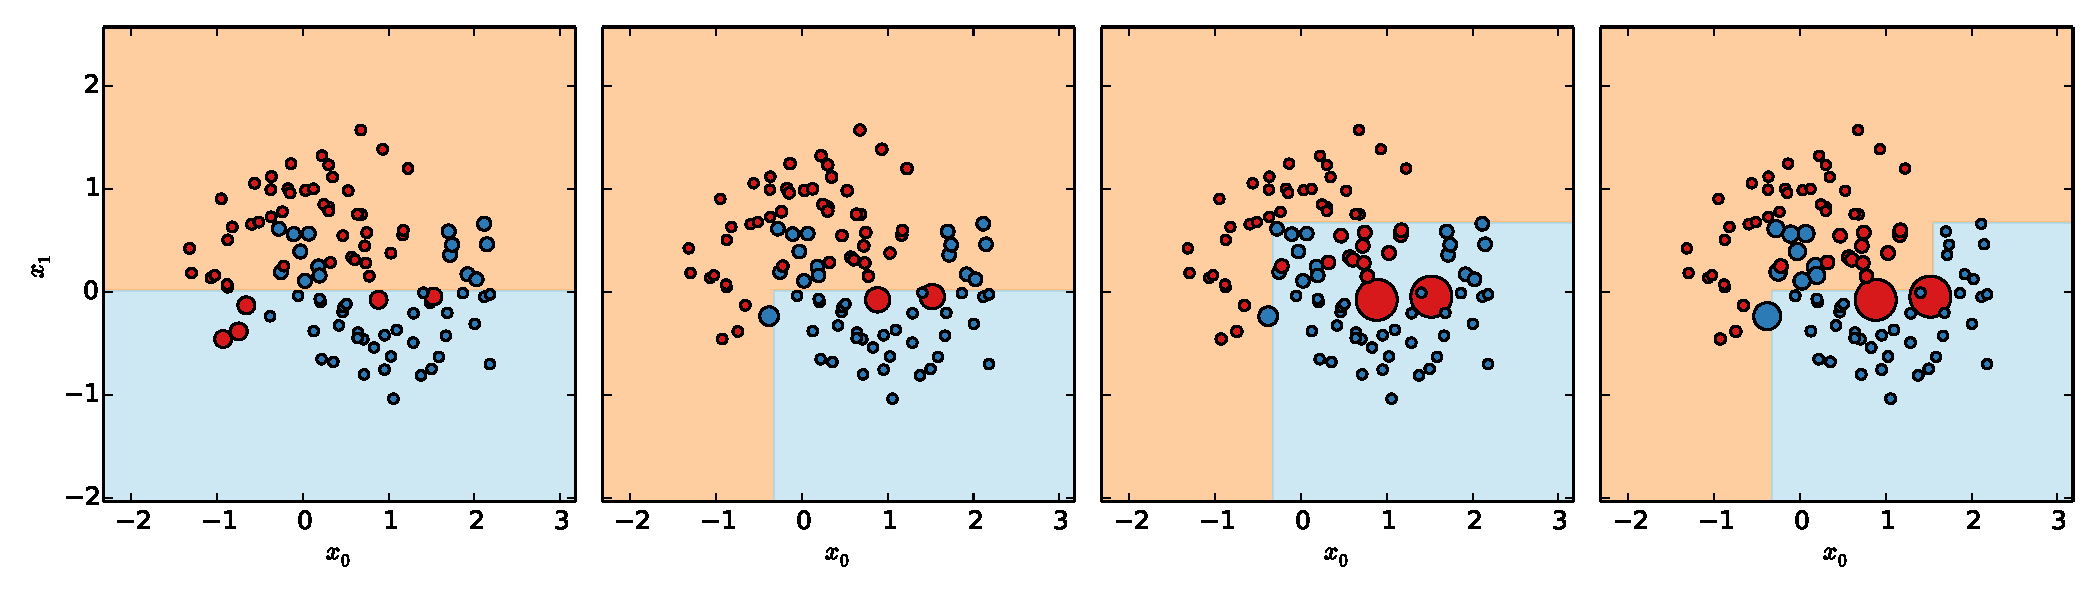
\includegraphics[width=\textwidth,trim=0 0 0 10, clip=true]{./images/adaboost.pdf}
        \end{figure}
    \end{block}

% sklearn footer
\tikzoverlay[text width=10cm] at (-0.2cm, 0.1cm) {
\begin{columns}[c]
\begin{column}{0.2\textwidth}
    \begin{figure}
      
\includegraphics[width=2em]{./images/scikit-learn-logo-thumb.png}
    \end{figure}
\end{column}
\begin{column}{1.0\textwidth}
    \vspace{-0.5cm}\hspace{-0.5cm}{\footnotesize \texttt{sklearn.ensemble.AdaBoostClassifier|Regressor}}
\end{column}
\end{columns}
};

\onslide<2->{
\tikzoverlayborder[text width=9cm] at (0.75cm,8cm) {
\begin{block}{Huge success}
\begin{itemize}
   \item Viola-Jones Face Detector (2001)
   \begin{figure}
      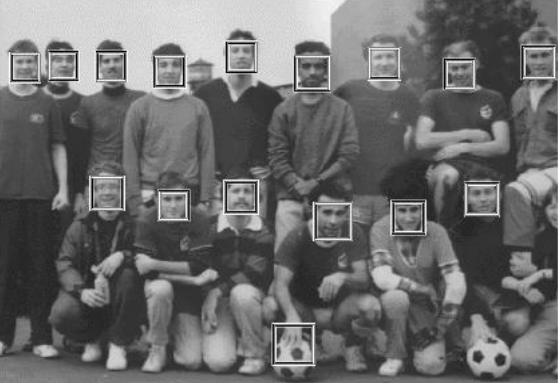
\includegraphics[scale=0.3]{./images/viola-jones.png}
    \end{figure}
   \item Freund \& Schapire won the Gödel prize 2003
\end{itemize}
\end{block}
};
}
\end{frame}

% Gradient Boosting =========================================================

\begin{frame}{Gradient Boosting [J. Friedman, 1999]}
    Statistical view on boosting \\
    {\footnotesize
    \begin{itemize}
        %\item Boosting fits an additive model in a forward stage-wise manner
        %\item AdaBoost optimizes an exponential loss function
        \item $\Rightarrow$ Generalization of boosting to arbitrary loss functions
    \end{itemize}
    }

    \begin{block}{Residual fitting}<2->
        \begin{figure}
           \centering
           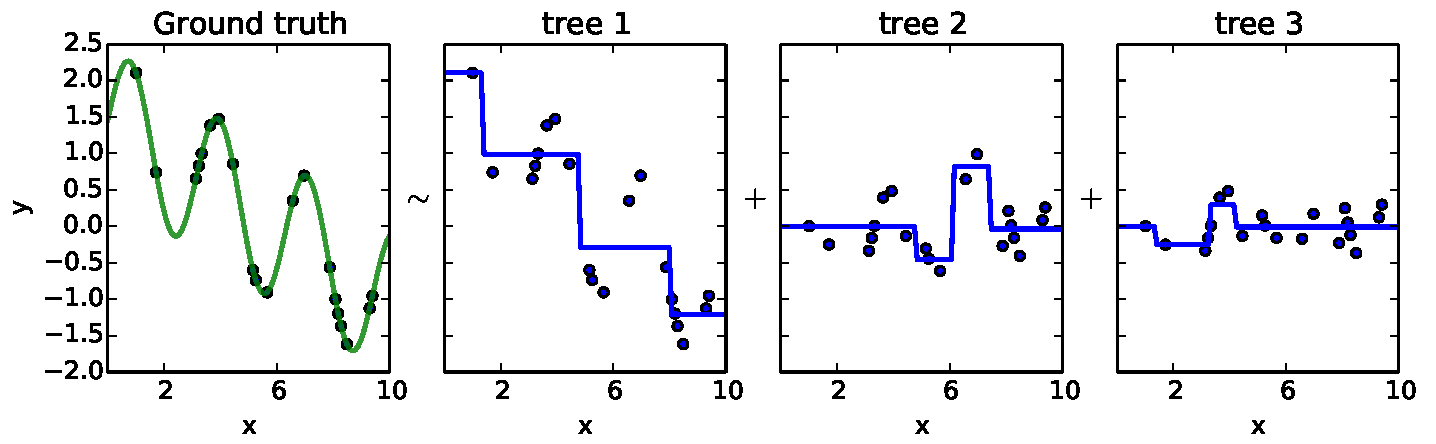
\includegraphics[width=\textwidth]{./images/residual_fitting_2.pdf}
        \end{figure}
    \end{block}

% sklearn footer
\onslide<2->{
\tikzoverlay[text width=10cm] at (-0.2cm,0.2cm) {
\begin{columns}[c]
\begin{column}{0.2\textwidth}
    \begin{figure}
      
\includegraphics[width=2em]{./images/scikit-learn-logo-thumb.png}
    \end{figure}
\end{column}
\begin{column}{1.0\textwidth}
    \vspace{-0.5cm}\hspace{-0.5cm}{\footnotesize \texttt{sklearn.ensemble.GradientBoostingClassifier|Regressor}}
\end{column}
\end{columns}
};
}
\end{frame}


% Gradient Boosting =========================================================

\begin{frame}{Functional Gradient Descent}
    \begin{block}{Least Squares Regression}
      \begin{itemize}
        \item Squared loss: $L(y_i,\;f(\mathbf{x}_i)) = (y_i - f(\mathbf{x}_i))^2$
        \item The residual $\sim$ the (negative) gradient $\frac{\partial L(y_i,\;f(\mathbf{x}_i))}{\partial f(\mathbf{x}_i)}$
      \end{itemize}
    \end{block}

    \begin{block}{Steepest Descent}<2->
      \begin{itemize}
        \item Regression trees approximate the (negative) gradient
        \item Each tree is a successive gradient descent step
      \end{itemize}
    \end{block}
    \vspace{-0.5cm}
    \begin{columns}[c]<2->
      % \begin{column}{.25\textwidth}
      %   \begin{figure}
      %     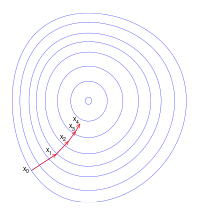
\includegraphics[scale=0.4,trim=0 0 10 0,clip=true]{./images/gradient-descent.png}
      %   \end{figure}
      % \end{column}
      \begin{column}{.5\textwidth}
        \begin{figure}
          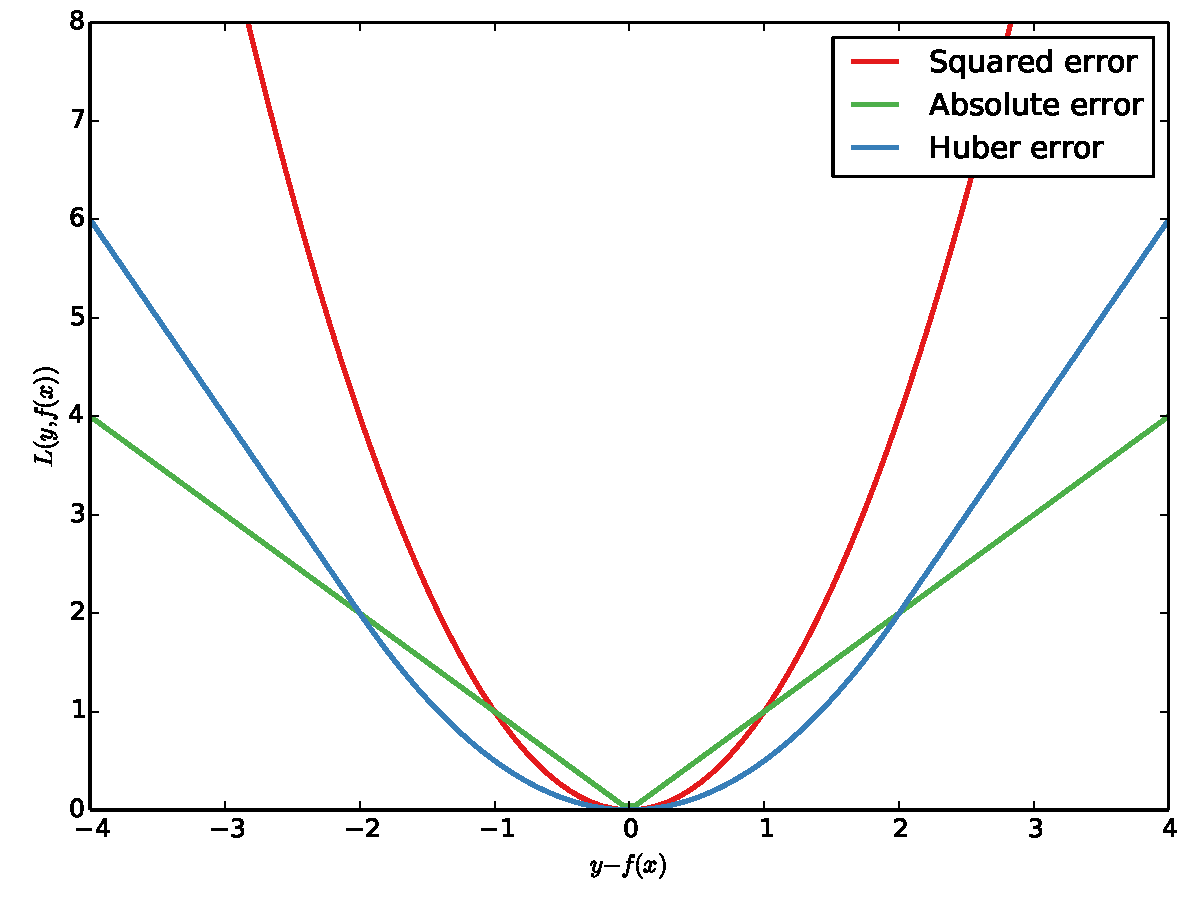
\includegraphics[scale=0.2]{./images/reg-loss-func.pdf}
        \end{figure}
      \end{column}
      \begin{column}{.5\textwidth}
        \begin{figure}
          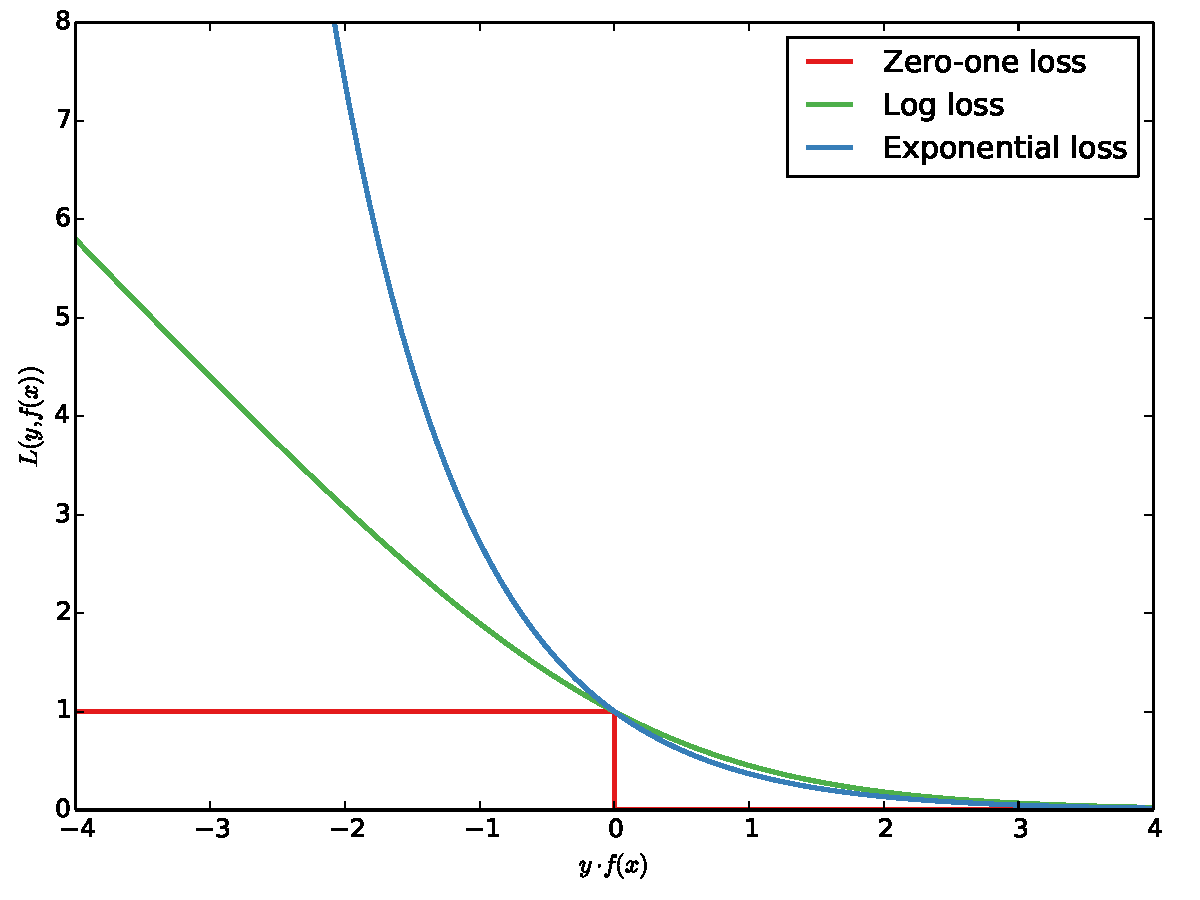
\includegraphics[scale=0.2]{./images/clf-loss-func.pdf}
        \end{figure}
      \end{column}
    \end{columns}

\end{frame}

\section{Gradient Boosting in scikit-learn}
% API and Docu =========================================================

\begin{frame}[plain]
  \begin{center}
    {\Large Notebook}\\
    \vspace{0.2cm}
    \href{https://github.com/pprett/pydata-gbrtm-tutorial}{https://github.com/pprett/pydata-gbrt-tutorial}\\
  \end{center}
\end{frame}

\section{Use Case: California Housing}

\end{document}


